\documentclass[11pt,a4paper]{article}
\usepackage[utf8]{inputenc}
\usepackage[T1]{fontenc}
\usepackage{mathptmx}
\usepackage{courier}
\usepackage[margin=0.8in]{geometry}
\usepackage{amsmath,amssymb}
\usepackage{booktabs,tabularx}
\usepackage[shortlabels]{enumitem}
\usepackage{microtype}
\usepackage[dvipsnames]{xcolor}
\usepackage[colorlinks=true,linkcolor=NavyBlue,citecolor=NavyBlue,urlcolor=NavyBlue]{hyperref}
\hypersetup{pdftitle={SAFE-Judge: Stage 2 Initial Pilot},pdfauthor={Ayush Ahuja}}
\usepackage{titlesec}
\usepackage{graphicx}
\usepackage{float}
\usepackage[font=small,labelfont=bf]{caption}
\titleformat{\section}{\large\bfseries}{\thesection}{0.6em}{}
\titleformat{\subsection}{\normalsize\bfseries}{\thesubsection}{0.5em}{}
\titlespacing*{\section}{0pt}{1.3ex}{0.6ex}
\titlespacing*{\subsection}{0pt}{1.0ex}{0.4ex}
\setlist{itemsep=1pt,topsep=3pt,parsep=0pt}
\setlength{\parskip}{2pt}
\setlength{\parindent}{0pt}
\setlength{\textfloatsep}{8pt}
\setlength{\intextsep}{6pt}
\newcolumntype{Y}{>{\raggedright\arraybackslash}X}
\newcolumntype{P}[1]{>{\raggedright\arraybackslash}p{#1}}
\graphicspath{{figures/stage2/}}
% Generated from validated pilot artifacts; rerun scripts/build_stage2_report.py.
\newcommand{\PilotAccuracy}{79.40}
\newcommand{\PilotFone}{0.7368}
\newcommand{\PilotBrier}{0.1485}
\newcommand{\PilotECE}{0.0688}
\newcommand{\PilotQueryAccuracy}{79.46}
\newcommand{\PilotScoreMinutes}{33.12}
\newcommand{\PilotProcessMinutes}{43.60}
\newcommand{\PilotPrepMinutes}{13.70}
\newcommand{\PilotThroughput}{4.66}
\newcommand{\PilotPeakAllocated}{3.91}
\newcommand{\PilotPeakReserved}{4.69}
\newcommand{\PilotGPUVRAM}{14.56}
\newcommand{\PilotTemperature}{1.6245}
\newcommand{\PilotReviewed}{50}
\newcommand{\PilotManifestHash}{e812a7e76cc4b3e87e62f34dd73c05ee108d7b09b15a1381f3ca13ee8610ec20}
\newcommand{\PilotPredictionHash}{c321f8374496f5c48deaf51c21e8ba55f29ffa446a7ed2e0ad49a1bb9b86dc65}
\newcommand{\PilotModelRevision}{851bf6e806efd8d0a36b00ddf55e13ccb7b8cd0a}
\newcommand{\PilotPipelineHash}{f3c066f0e9318a72ab3351d1bf237eb351b32c78d02534cff3f4439f89761d0d}
\newcommand{\PilotMassMean}{0.9988}
\newcommand{\PilotMassMin}{0.9977}
\newcommand{\PilotRepeatMean}{0.000680}
\newcommand{\PilotRepeatMax}{0.004161}
\newcommand{\PilotRepeatSeconds}{31.81}
\newcommand{\PilotHFCache}{9.33}
\newcommand{\PilotCorpusCache}{4.11}
\newcommand{\PilotBaselineRows}{%
Qwen3.5-4B & 79.40 & 0.7368 & 0.1485 & 0.0688 \\
Always non-relevant & 72.99 & 0.4219 & 0.2701 & 0.2701 \\
Always relevant & 27.01 & 0.2127 & 0.7299 & 0.7299 \\
}
\newcommand{\PilotIntervalRows}{%
Accuracy & 0.7558 & 0.8294 \\
Macro-F1 & 0.6778 & 0.7828 \\
Brier score & 0.1224 & 0.1774 \\
ECE (10 probability bins) & 0.0435 & 0.1104 \\
Query-mean accuracy & 0.7544 & 0.8332 \\
Accuracy gain over always non-relevant & 0.0059 & 0.1126 \\
}
\newcommand{\PilotGradeRows}{%
0 & 5,158 & 55.70 & 424 & 8.22 \\
1 & 1,601 & 17.29 & 501 & 31.29 \\
2 & 1,804 & 19.48 & 691 & 38.30 \\
3 & 697 & 7.53 & 292 & 41.89 \\
}
\newcommand{\PilotThresholdRows}{%
0.50 & 9,260 & 100.00 & 20.60 & 20.60 \\
0.70 & 7,756 & 83.76 & 15.90 & 13.32 \\
0.80 & 6,690 & 72.25 & 13.06 & 9.44 \\
0.90 & 4,632 & 50.02 & 9.78 & 4.89 \\
0.95 & 2,389 & 25.80 & 7.33 & 1.89 \\
0.99 & 23 & 0.25 & 0.00 & 0.00 \\
}
\newcommand{\PilotCalibrationRows}{%
Raw & 79.76 & 0.7413 & 0.1437 & 0.0626 \\
Temperature scaled & 79.76 & 0.7413 & 0.1417 & 0.0753 \\
}
\newcommand{\PilotManualAnalysis}{%
I reviewed 50 unique errors across 31 queries: 27 false positives and 23 false negatives.
\begin{table}[H]\centering\small
\caption{Primary categories in the 50 personally reviewed disagreements. FP/FN use the official binary labels.}\label{tab:manual}
\begin{tabular}{@{}lrrrr@{}}\toprule Category & Count & Share (\%) & FP & FN \\\midrule
Judgment disagreement & 23 & 46 & 12 & 11 \\
Incomplete answer & 10 & 20 & 10 & 0 \\
Subtle relevance & 9 & 18 & 0 & 9 \\
Keyword distraction & 4 & 8 & 4 & 0 \\
Entity mismatch & 3 & 6 & 1 & 2 \\
Domain vocabulary & 1 & 2 & 0 & 1 \\
\bottomrule\end{tabular}\end{table}
The sample contains 19 high-confidence disagreements (confidence at least 0.90). Category shares describe this diagnostic sample, not the prevalence of causes in all 1,908 errors.
}


\begin{document}
\begin{center}
{\small COL764: Information Retrieval and Web Search}\\[4pt]
{\Large\bfseries Calibrated and Selective LLM Relevance Assessment\\[2pt] under Domain Shift}\\[6pt]
{\large Stage 2 Report: Initial Pilot}\\[8pt]
\begin{tabular}{rl}
\textbf{Name:} & Ayush Ahuja \\
\textbf{Entry No.:} & 2023CS50911 \\
\end{tabular}
\end{center}
\vspace{-2pt}\hrule\vspace{6pt}

\textbf{Pilot summary.} A frozen, 4-bit Qwen3.5-4B assessor was evaluated on all
9,260 judged TREC DL 2019 passage pairs from 43 queries. It achieved
\PilotAccuracy\% accuracy and \PilotFone{} macro-F1. At confidence 0.90,
50.02\% of pairs were accepted, with 9.78\% error among accepted pairs. A
query-disjoint temperature-scaling experiment improved Brier score but worsened
10-bin ECE. Scoring took \PilotScoreMinutes{} minutes on one Tesla T4.
These results establish a working pilot and motivate further selective-assessment
experiments; they do not establish a conformal guarantee or domain-shift robustness.

\section{Research Question and Pilot Scope}
Human relevance judgments support reusable IR test collections, but producing them
is expensive. The project asks whether a compact LLM can identify which of its
judgments need human review, reducing annotation effort while preserving label
quality and the ranking of retrieval systems. The intended final method,
\textbf{SAFE-Judge}, combines confidence-based escalation with query-level risk
calibration and evaluation under web-to-biomedical domain shift.

The present pilot tests a narrower question: \emph{does the confidence of a frozen
compact assessor identify a useful trade-off between automatic-label coverage and
errors, and what changes when its probabilities are temperature-scaled?}
The hypotheses about formal risk control, system-ranking fidelity and shifted-domain
performance from Stage 1 remain untested.

\textbf{Change from the proposal.} The Stage 1 plan described an approximately 3B,
graded assessor adapted with QLoRA. This pilot uses a post-trained 4B model, a
binary relevance rubric and frozen 4-bit inference. No adapter training or teacher
generation was performed. The scope isolates scoring, calibration and evaluation
before introducing training. Four-bit loading is quantized inference, not QLoRA.
The measured memory use verifies feasibility for this inference workload on a
single approximately 16\,GB GPU; it does not establish training feasibility.

\section{Closest Work and Response to Feedback}
\textbf{LARA}~\cite{lara} selects useful documents for manual assessment under a
fixed budget and learns to calibrate/debias LLM probabilities. It is the closest
planned comparison for annotation allocation and system-ranking fidelity.
\textbf{DIRAS}~\cite{diras} fine-tunes compact open annotators using stronger-model
supervision and motivates the later teacher/student experiment. Neither has been
reproduced in this pilot.

\textbf{Oosterhuis et al. (KDD 2024)}~\cite{oosterhuis}, added in response to the
Stage 1 feedback, already combine generated relevance annotations with reliable
labels using prediction-powered inference and conformal risk control to construct
confidence intervals for IR metrics. Formal uncertainty control for generated
relevance judgments is therefore not novel by itself. The proposed distinction is
\emph{which labels to accept or escalate}, with explicit class/query diagnostics,
matched annotation budgets and transfer evaluation. Metric intervals and an
escalation policy have different outputs; both require downstream validation.
The bootstrap intervals in this report quantify uncertainty in observed pilot
metrics and are not a reproduction of their metric-correction method.

The proposed teacher is
\texttt{meta-llama/Llama-3.3-70B-Instruct}, proposed only for later training-label generation.
A one-time HPC run is proposed for at most 10,000 MS MARCO training pairs;
the allocation and API fallback are specified in the remaining budget.

\section{Data and Experimental Protocol}
\subsection{Judged pool and relevance definition}
The experiment uses \texttt{msmarco-passage/trec-dl-2019/judged} from
\texttt{ir\_datasets}. TREC DL supplies the queries and human judgments; the passage
text comes from the shared MS MARCO collection~\cite{trecdl,irds}.
All 9,260 unique judged query--passage pairs from all 43 judged queries are included.
Unjudged pairs are excluded. No query or per-query pair sampling is applied.
The full 8.8-million-passage corpus is not scored: it is scanned during preparation
to recover the required texts. This does not build a retrieval index.

Grades 0 (irrelevant) and 1 (related but not answering the query) map to binary
non-relevance; grades 2 (highly relevant) and 3 (perfectly relevant) map to relevance.
There are 6,759 non-relevant and 2,501 relevant pairs, so the relevant fraction is
27.01\%. This imbalance makes accuracy alone insufficient.
The judged pool is a benchmark pool, not a representative sample of every possible
query--passage pair.

\subsection{Prompt and probability extraction}
The assessor is \texttt{Qwen/Qwen3.5-4B}~\cite{qwen}. Its native chat template is
used with thinking disabled.
The system message treats the query and passage as data and requires exactly
\texttt{Yes} or \texttt{No}. The user message states the grade cutoff explicitly,
encloses the query and passage in separate tags, and says that topical overlap
alone is insufficient for relevance. No official gold grade is supplied to the model.
The complete prompt is included in the source release.

Let $z_Y,z_N$ denote the next-token logits for the canonical Yes/No continuations.
The score, predicted label and confidence are
\[
 p_i=\frac{\exp(z_Y)}{\exp(z_Y)+\exp(z_N)},\qquad
 \hat y_i=\mathrm{I}(p_i\geq0.5),\qquad c_i=\max(p_i,1-p_i).
\]
Here, $\mathrm{I}(E)$ is the indicator function: it equals 1 when condition $E$
is true and 0 otherwise.
The implementation uses a float32 softmax for numerical stability. It verifies that
each answer is one token at the actual answer boundary and projects only the final
hidden state to vocabulary logits. It does not sample answers or generate explanations.
The score is conditional on the two answer tokens, rather than an independently
validated probability of correctness.

Inputs have a 512-token cap, with only the document prefix eligible for truncation;
query, rubric and assistant boundary are preserved. In this run \textbf{no pairs
were truncated}: inputs ranged from 162 to 452 tokens (mean 226.30).
The full-vocabulary probability mass on Yes/No averaged \PilotMassMean{}, with
minimum \PilotMassMin{}, supporting adherence to the requested answer format.
This does not establish semantic correctness or calibration.

\subsection{Execution and analysis}
The model uses NF4 4-bit weights with double quantization, FP16 computation,
evaluation mode and SDPA attention. Batches 1, 2, 4, 8 and 16 are timed on 32
long inputs selected by character length without consulting gold labels. Batch 8
had the highest observed throughput and was used for the main run. This is a single
timing probe, not a repeated performance benchmark.

The aggregate pilot results and raw confidence sweeps use all 43 queries for
description. A separate temperature-scaling comparison holds out 33 queries
(7,328 pairs) from 10 calibration queries (1,932 pairs), using seed 42.
It estimates calibration performance on unseen queries within this collection.
No future threshold should be selected on the full-pool curves and then claimed
to have held-out performance on the same pairs.

\section{Label Quality and Query-Level Uncertainty}
Table~\ref{tab:baseline} compares the frozen assessor with constant-label reference
points. Accuracy is \PilotAccuracy\%, versus 72.99\% for always non-relevant:
a gain of 6.40 percentage points. Macro-F1 improves from 0.4219 to \PilotFone{}.
These constant baselines expose class imbalance; they do not replace the planned
classical active-learning, cross-encoder or recent LLM baselines.

\begin{table}[H]\centering\small
\caption{Full judged pool: 9,260 pairs, 43 queries. Lower Brier/ECE is better. ECE
uses 10 equal-width bins of $P(\mathrm{relevant})$.}\label{tab:baseline}
\begin{tabular}{@{}lrrrr@{}}\toprule
Method & Accuracy (\%) & Macro-F1 & Brier & ECE \\\midrule
\PilotBaselineRows
\bottomrule\end{tabular}
\end{table}

Uncertainty is estimated with 10,000 percentile bootstrap resamples of complete
queries, seed 42 (Table~\ref{tab:intervals}). Pairs within a query are kept together.
For each resample, pooled confusion counts and probability metrics are recomputed.
The paired accuracy-gain interval uses the same resampled queries for both methods.
Its lower endpoint is above zero, but this descriptive comparison does not establish
superiority over the stronger baselines or on another domain.

\begin{table}[H]\centering\small
\caption{95\% whole-query bootstrap intervals. Entries are fractions, including
the accuracy difference; 0.01 corresponds to one percentage point.}\label{tab:intervals}
\begin{tabular}{@{}lrr@{}}\toprule Metric & Lower & Upper \\\midrule
\PilotIntervalRows
\bottomrule\end{tabular}
\end{table}

\begin{figure}[H]\centering
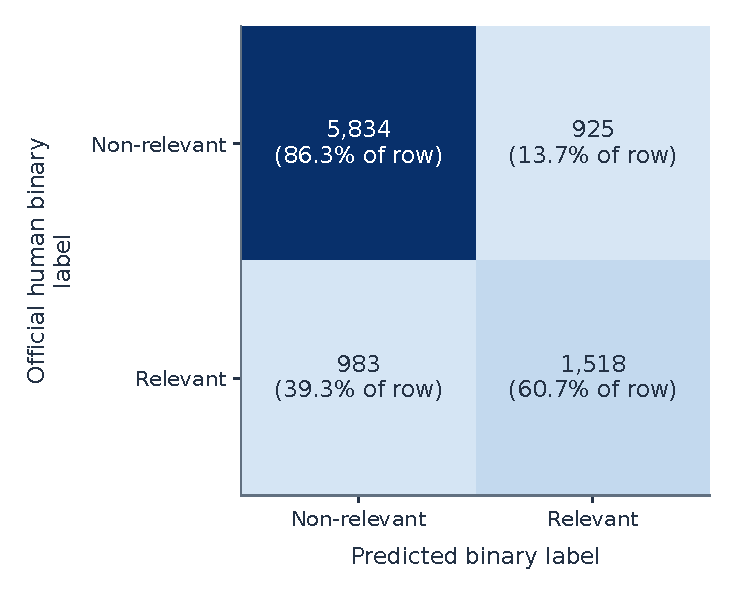
\includegraphics[width=.64\textwidth]{confusion_matrix.pdf}
\caption{Full-pool confusion matrix. Counts are accompanied by percentages within
each human-label row. Relevant-pair recall is 60.70\%; non-relevant-pair recall is
86.30\%. There are 925 false positives and 983 false negatives.}\label{fig:confusion}
\end{figure}

\section{Selective Assessment: Coverage and Error}
For acceptance $a_i(\lambda)=\mathrm{I}(c_i\geq\lambda)$, define coverage $C$,
selective risk $R$ and auto-error $A$ by
\[
C=\frac{\sum_i a_i}{N},\qquad
R=\frac{\sum_i a_i\mathrm{I}(\hat y_i\neq y_i)}{\sum_i a_i},\qquad
A=\frac{\sum_i a_i\mathrm{I}(\hat y_i\neq y_i)}{N}=CR.
\]
Selective risk is undefined when no pairs are accepted. Each prediction at 0.5 is
counted once, with ties assigned to relevant. The sweep uses 101 confidence
thresholds from 0.50 to 1.00; selected points appear in Table~\ref{tab:thresholds}.

\begin{table}[H]\centering\small
\caption{Descriptive full-pool operating points. These are not held-out choices
or guaranteed operating bounds.}\label{tab:thresholds}
\begin{tabular}{@{}rrrrr@{}}\toprule
Threshold & Accepted pairs & Coverage (\%) & Selective risk (\%) & Auto-error (\%) \\\midrule
\PilotThresholdRows
\bottomrule\end{tabular}
\end{table}

\begin{figure}[H]\centering
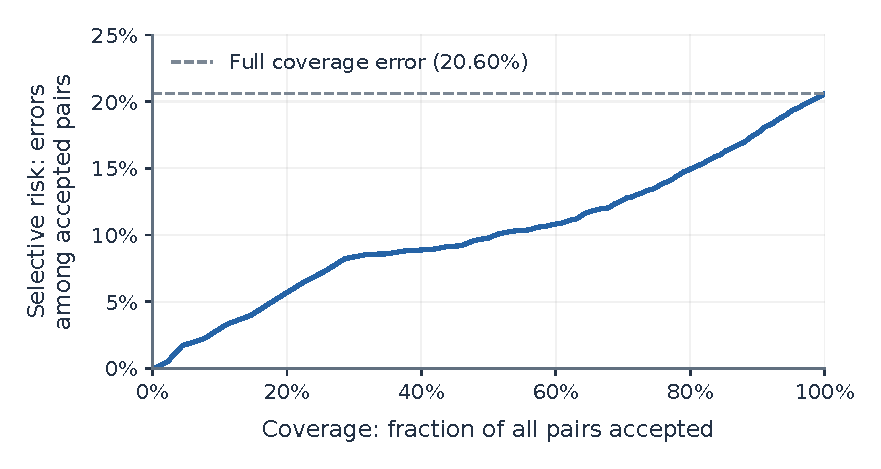
\includegraphics[width=.64\textwidth]{risk_coverage.pdf}
\caption{Overall confidence sweep. At $\lambda=0.90$, 4,632 pairs (50.02\%)
are accepted and 453 are wrong: 9.78\% selective risk and 4.89\% auto-error.
The zero-error endpoint at 0.99 contains only 23 pairs and is not evidence of zero
future risk.}\label{fig:risk}
\end{figure}

\begin{figure}[H]\centering
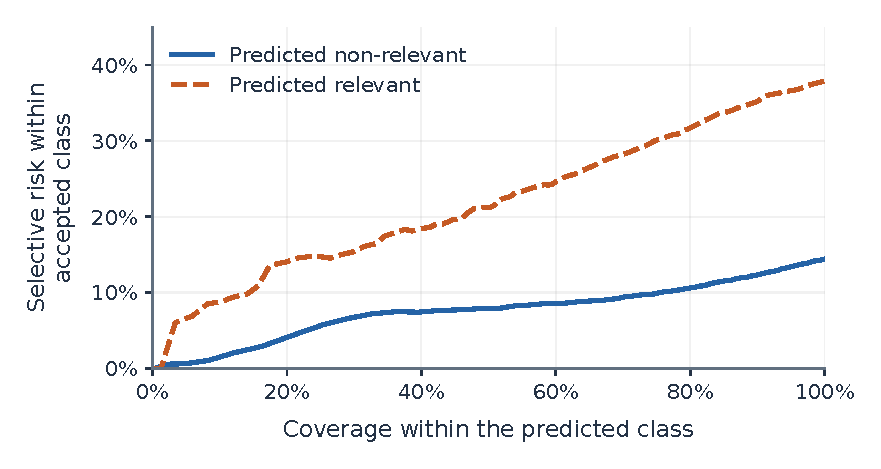
\includegraphics[width=.64\textwidth]{class_risk_coverage.pdf}
\caption{Class-specific curves. Each coverage denominator is the size of that
\emph{predicted} class (2,443 relevant; 6,817 non-relevant). At full coverage,
37.86\% of relevant predictions are wrong, versus 14.42\% of non-relevant predictions.
The different denominators mean equal class coverage does not imply equal pair counts.}\label{fig:classrisk}
\end{figure}

\section{Calibration Experiment}
Temperature scaling~\cite{guo} transforms the conditional logit difference using
$p_T=\sigma((z_Y-z_N)/T)$. A fixed grid $T=2^{j/10}$ for
$j=-30,\ldots,30$ minimizes binary negative log-likelihood on the 10 calibration
queries only. The selected temperature is $T=\PilotTemperature$.
Both methods in Table~\ref{tab:calibration} are evaluated on exactly the same 33
held-out queries and 7,328 pairs.

\begin{table}[H]\centering\small
\caption{Query-disjoint calibration comparison. Lower Brier/ECE is better.}
\label{tab:calibration}
\begin{tabular}{@{}lrrrr@{}}\toprule
Method & Accuracy (\%) & Macro-F1 & Brier & ECE \\\midrule
\PilotCalibrationRows
\bottomrule\end{tabular}
\end{table}

Brier improves from 0.1437 to 0.1417 (about 1.37\% relative), while ECE increases
from 0.0626 to 0.0753. This is a mixed result: minimizing calibration-set
log-loss does not guarantee improvement in a fixed-bin ECE on different queries.
Accuracy and macro-F1 remain unchanged because a positive temperature preserves
the decision boundary. It also preserves the ordering of absolute logit differences,
so it cannot improve the risk--coverage ordering except for numerical ties. It
changes probability values and fixed-threshold acceptance, not the underlying
ordering of uncertain pairs. Only one query split was tested.

\begin{figure}[H]\centering
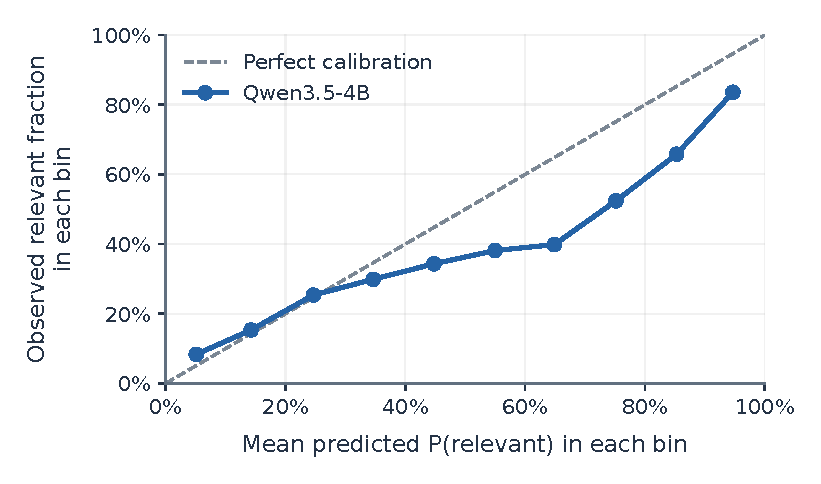
\includegraphics[width=.61\textwidth]{reliability.pdf}
\caption{Raw probability reliability on all 43 queries. Each point uses one of
10 equal-width probability bins. Points below the diagonal indicate overestimation
of relevance probability in that bin. Bins contain different numbers of pairs.}
\label{fig:reliability}
\end{figure}

\begin{figure}[H]\centering
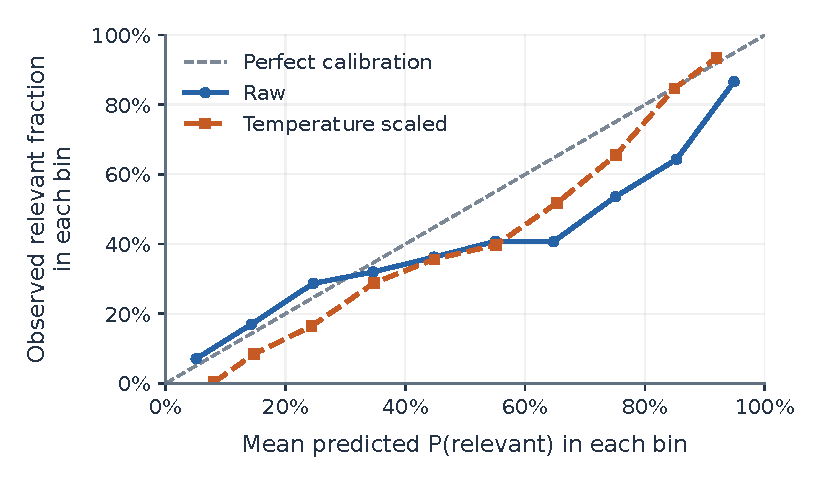
\includegraphics[width=.61\textwidth]{calibration_reliability.pdf}
\caption{Raw and temperature-scaled reliability on the 33 held-out queries only.
Bin membership changes after scaling. This comparison must not be confused with
the full-pool reliability curve above.}\label{fig:calibration}
\end{figure}

\section{Manual Failure Analysis}
Fifty unique errors were selected from the 1,908 benchmark disagreements using
round-robin sampling over shuffled query/error-type/confidence strata, seed 42.
Each review records a primary category and passage-based notes. The sample is
diagnostic rather than prevalence-weighted.

\PilotManualAnalysis

\textbf{Main findings.} Judgment disagreement was the largest category (23/50),
followed by incomplete answers (10) and subtle relevance (9). All ten incomplete-answer
cases were false positives; all nine subtle-relevance cases were false negatives.
This separates over-crediting related text from missing an indirect answer.
The 23 judgment-disagreement flags record my assessment, not an adjudicated
correction of the benchmark: the official grades and all quantitative results remain
unchanged. No inputs were truncated in this run.

\textbf{Representative examples, summarized from my notes.}
\begin{enumerate}[leftmargin=*,itemsep=4pt]
\item \textbf{Keyword distraction} (query 962179, passage 8785374; FP).
For ``when was the Salvation Army founded,'' the passage names William and Catherine
Booth as founders but gives no date. The model accepted an answer to \emph{who}
rather than \emph{when} (official grade 0).
\item \textbf{Incomplete answer} (query 1110199, passage 2796199; FP).
For ``what is wifi vs bluetooth,'' the passage names both technologies and describes
Wi-Fi, but does not compare them. I considered the official grade 1
appropriate; related information was over-credited as an answer.
\item \textbf{Subtle relevance} (query 1124210, passage 7228448; FN).
For ``tracheids are part of \_\_\_\_\_,'' the passage places vessels and tracheids
within a discussion of water transport in the xylem. I identified an
implicit answer that the model rejected (official grade 2).
\item \textbf{Entity mismatch} (query 443396, passage 8769489; FP).
For ``lps laws definition,'' the passage uses LPS for ``large polyp stony'' coral.
The shared acronym refers to the wrong subject rather than the query's legal
sense (official grade 0).
\item \textbf{Domain vocabulary} (query 1114646, passage 444374; FN).
The query asks what Famvir is prescribed for, while the passage discusses
famciclovir without naming Famvir. I flagged brand--generic terminology
matching as a possible explanation, not a proven internal model mechanism
(official grade 2).
\item \textbf{Judgment disagreement} (query 148538, passage 2713526; FN).
For ``difference between rn and bsn,'' the passage discusses biomedical engineering
degrees. I questioned its official grade 2 and considered the model's
non-relevant response defensible. The official label was retained for scoring.
\end{enumerate}
The complete review is supplied as \nolinkurl{reports/failure_review.csv}.
Each of its 50 rows includes passage text and my explanation. These observations motivate
clearer answer-completeness checks, acronym/terminology diagnostics and separate
analysis of debatable gold judgments in the next stage.

\section{Efficiency and Numerical Consistency}
\begin{table}[H]\centering\small
\caption{Measured Colab pilot consumption. GiB uses $2^{30}$ bytes; cache GB uses
$10^9$ bytes. These measurements are separate from the remaining project budget.}
\begin{tabularx}{\textwidth}{@{}Y r@{}}\toprule
Measurement & Recorded value \\\midrule
GPU / available VRAM & Tesla T4 / \PilotGPUVRAM{} GiB \\
Main scoring time / throughput & \PilotScoreMinutes{} min / \PilotThroughput{} pairs/s \\
Inference process, including loading, tuning and repeat & \PilotProcessMinutes{} min \\
Dataset preparation wall time & \PilotPrepMinutes{} min \\
Peak allocated / reserved VRAM during main run & \PilotPeakAllocated{} / \PilotPeakReserved{} GiB \\
Hugging Face / dataset cache & \PilotHFCache{} / \PilotCorpusCache{} GB \\
\bottomrule\end{tabularx}
\end{table}

The main-run memory statistics were reset after batch tuning. They are PyTorch
allocation statistics, not total device usage. Process time excludes notebook
installation and corpus preparation; it is not scheduler-accounted allocation time.
Drive snapshots were taken approximately every 120 seconds after completed batches.
The full main run averaged \PilotThroughput{} pairs/s, whereas the long-input tuning
probe reached 3.61 pairs/s (Figure~\ref{fig:batch}).

\begin{figure}[H]\centering
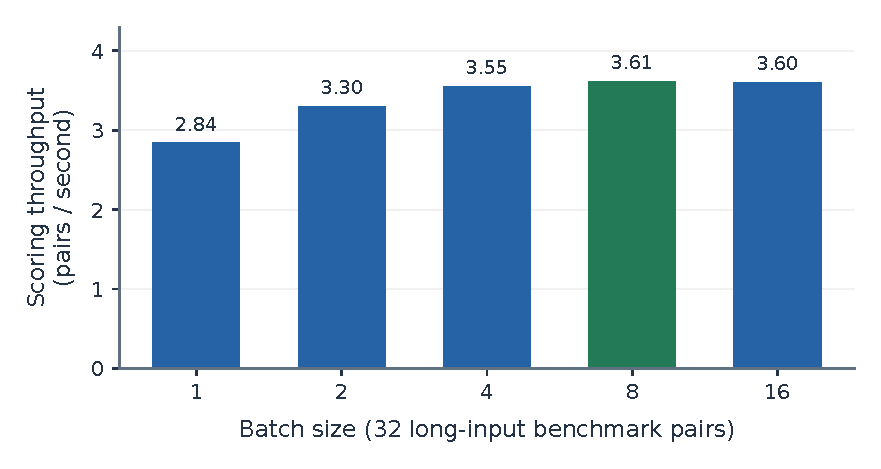
\includegraphics[width=.64\textwidth]{batch_throughput.pdf}
\caption{One timing probe per batch size on 32 long inputs. Batch 8 was marginally
faster than 16, so no statistically supported speed advantage is claimed between
them. These are throughput probes, not substantive method ablations.}\label{fig:batch}
\end{figure}

After the main run, the first 100 frozen pairs were rescored at batch size 1 in
\PilotRepeatSeconds{} seconds. All binary labels agreed. The mean absolute
probability difference was \PilotRepeatMean{}, with maximum \PilotRepeatMax{}.
This is a within-session numerical/batching check on 100 pairs, not a full independent
rerun or stochastic self-consistency experiment.

\section{Remaining Resource Budget}
The following caps cover work \emph{beyond this completed pilot}. Main experiments
are planned on one V100 with at least 16\,GB VRAM, requested through the IIT Delhi
HPC project \texttt{col764.course}.

\begin{table}[H]\centering\small
\caption{Proposed remaining resource caps. The API route is a fallback to the local teacher run.}
\begin{tabularx}{\textwidth}{@{}P{3.5cm} Y@{}}\toprule
Resource & Planned allocation / cap \\\midrule
Main experiments & One V100, at least 16\,GB VRAM; 50 GPU-hours total for assessor inference, adapter experiments, baselines and reruns. \\[4pt]
Teacher generation & \texttt{meta-llama/Llama-3.3-70B-Instruct}, 4-bit; one A100 80\,GB GPU for at most 6 GPU-hours and 10,000 MS MARCO training pairs. \\[4pt]
Optional API fallback & OpenAI GPT-6.1 Sol through Batch API; approximately US\$20 in credits, with a US\$20 spending cap and up to 10,000 pairs, instead of the local teacher run. \\[4pt]
Annotation & No new paid judgments (US\$0). Existing official qrels supply simulated calibration and escalation labels; 50 failure reviews are complete. \\[4pt]
Retrieval indexing & No new corpus index; reuse existing training candidates and official TREC runs. \\
\bottomrule\end{tabularx}
\end{table}

The local teacher output is limited to 64 tokens per pair; the API input cap is
1,024 tokens per pair. The API route uses low reasoning effort, with billed reasoning
included in the output-token budget. A 100-pair probe will measure label quality,
token use and cost before setting the API output limit and affordable pair count.
The API budget does not guarantee 10,000 completed labels. Generation stops at the
pair, compute or spending cap, whichever is reached first. Teacher labels are used only for training, with
evaluation retained against official human labels. Adapter-training memory and
teacher throughput will be checked on small batches before the full jobs.
The 10,000-pair allowance is an initial adaptation budget. Nested training subsets
of 2,000, 5,000 and 10,000 pairs, separated from development and test queries, will
measure the effect of training-data size. Labels are generated once and reused
across subsets and training seeds. Larger-scale generation will be considered only
if the development learning curve still improves and the budget is revised.

The pilot rate implies about 0.552 scoring hours for another 9,260 pairs on the
measured T4 workload, excluding setup. The 50-hour allowance includes other models,
training and reruns; it is a planning cap rather than a measured V100 runtime.
Saved probabilities will be reused for CPU-based calibration, query splits,
bootstrap analysis and system-ranking evaluation.

\section{Statistical Plan and Remaining Experiments}
\textbf{Comparisons.} Freeze prompts, datasets, calibration splits and evaluation
metrics before final testing. Compare the same assessor with raw confidence,
post-hoc calibration and the proposed escalation rule; add the classical lexical
active learner, a calibrated cross-encoder and LARA. Reproduce Oosterhuis et al.'s
metric-interval method separately and report interval coverage/width. Compare label
allocation methods at matched human budgets that include calibration/seed labels.

\textbf{Uncertainty and significance.} For Stage 3, confidence intervals for differences
between methods will use 10,000 bootstrap samples of complete queries. Each comparison
will use the same sampled queries. Official TREC runs will be evaluated using full
human labels and mixed automatic/human labels. Average system scores, rankings and
Kendall's $\tau$ between the two rankings will be recalculated in each sample.
All comparisons will use the same binary relevance scale and treatment of unjudged
documents.

Per-query effectiveness differences will be tested using a two-sided paired
randomization test. Main comparisons will be chosen before testing, and p-values
will be adjusted for multiple tests. Overlapping query splits will check sensitivity
to the split; they are not independent repetitions.

\textbf{Ablation experiments.} Two design choices will be tested: (i) one confidence
threshold versus separate thresholds for predicted relevant/non-relevant pairs;
and (ii) calibration using whole queries versus individual pairs. Assessor scores
and total human-label budgets will remain fixed. The number of target-domain
calibration queries will also be varied. Batch-size timing and the 100-pair repeat
measure speed and numerical consistency separately.

\subsection{Risk-control feasibility and revised hypothesis}
Conformal risk control (CRC) requires a precisely defined bounded, monotone loss
and exchangeability assumptions~\cite{crc}. For bounded loss $B=1$, its standard
correction uses
\[
\frac{n\widehat R(\lambda)+1}{n+1}\leq\alpha.
\]
For query-level calibration, define the loss per query before averaging; an equal
query-weighted guarantee is not automatically a guarantee for pair-weighted loss.
At $n=10$ and $\alpha=0.05$, even zero empirical loss gives $1/11>0.05$.
Thus the Stage 1 suggestion that ten target queries suffice for nontrivial vanilla
CRC at this risk level must be revised. Increase calibration size, justify another
valid loss/bound, or fall back to full escalation. Controlling auto-error alone
does not bound error among accepted labels, especially within a predicted class.
CRC controls expected loss under its assumptions, not success on 95\% of arbitrary
random splits or automatic validity under domain shift.

\textbf{Primary hypothesis for Stage 3.} At matched total human-label budgets,
query-calibrated selective assessment will reduce worst-predicted-class error at
useful coverage while preserving system-ranking fidelity on held-out queries.
The intended targets remain auto-error at most 0.05, at least 50\% coverage and
Kendall's $\tau\geq0.90$, subject to a feasible calibration design. None follows
from the descriptive point at threshold 0.90 in this pilot.

\textbf{Backoff.} If coverage becomes too small or source-calibrated errors fail
under biomedical shift, report a calibration-under-shift study instead: measure
the trade-off as target calibration data increases, compare active versus random
annotation selection, and identify systematic high-confidence errors. DL2020 and
TREC-COVID evaluation, training/teacher generation, the stronger baselines and
system-ranking experiments remain future work. Reserve blind audit topics before
any shifted-domain prompt or policy tuning.

\section{Limitations, Repository and AI Use}
This is one frozen model, one prompt, one quantization setting and one collection.
The model was not trained on project data, but public benchmark contamination in
its pretraining cannot be excluded. Binary labels discard differences within the
original grades, and official qrels can contain ambiguity. Aggregate curves are
descriptive; tiny accepted subsets have high uncertainty. The calibration comparison
uses one split, and ECE depends on its binning scheme. No system-ranking,
teacher-comparison or cross-domain result has been measured.

\textbf{Repository:} \url{https://github.com/Ayush-Ahuja/SAFE-Judge}.

\begin{samepage}
\textbf{AI-use statement.} AI assistance was used to implement scripts and prepare the
notebook, understand the papers and supporting technical material, draft the report, and investigate and fix bugs encountered during the work.
I designed the experiments, ran the Colab workflow,
analyzed the experimental results, and manually reviewed and categorized the 50
failures. The final experimental choices and interpretation
are my responsibility.

\end{samepage}

\small
\begin{thebibliography}{9}\setlength{\itemsep}{4pt}
\bibitem{lara} R.~Takehi, E.~M.~Voorhees, T.~Sakai and I.~Soboroff.
LLM-Assisted Relevance Assessments: When Should We Ask LLMs for Help?
\emph{SIGIR}, 2025. \url{https://doi.org/10.1145/3726302.3729916}.
\bibitem{diras} J.~Ni, T.~Schimanski, M.~Lin, M.~Sachan, E.~Ash and M.~Leippold.
DIRAS: Efficient LLM Annotation of Document Relevance for Retrieval Augmented Generation.
\emph{NAACL}, 2025. \url{https://aclanthology.org/2025.naacl-long.271/}.
\bibitem{oosterhuis} H.~Oosterhuis, R.~Jagerman, Z.~Qin, X.~Wang and M.~Bendersky.
Reliable Confidence Intervals for Information Retrieval Evaluation Using Generative A.I.
\emph{KDD}, 2024. \url{https://doi.org/10.1145/3637528.3671883}.
\bibitem{guo} C.~Guo, G.~Pleiss, Y.~Sun and K.~Q.~Weinberger.
On Calibration of Modern Neural Networks. \emph{ICML}, 2017.
\url{https://proceedings.mlr.press/v70/guo17a.html}.
\bibitem{crc} A.~N.~Angelopoulos, S.~Bates, A.~Fisch, L.~Lei and T.~Schuster.
Conformal Risk Control. \emph{ICLR}, 2024.
\url{https://arxiv.org/abs/2208.02814}.
\bibitem{trecdl} TREC. 2019 Deep Learning Track Guidelines.
\url{https://microsoft.github.io/msmarco/TREC-Deep-Learning-2019.html}.
\bibitem{irds} ir\_datasets. MS MARCO Passage dataset documentation.
\url{https://ir-datasets.com/msmarco-passage.html}.
\bibitem{qwen} Qwen Team. Qwen3.5-4B model card.
\url{https://huggingface.co/Qwen/Qwen3.5-4B}.
\end{thebibliography}
\normalsize

\appendix
\setlength{\intextsep}{6pt}
\captionsetup[figure]{skip=5pt}
\section{Additional Diagnostics}
Table~\ref{tab:grades} shows that the binary problem retains meaningful grade-specific
variation. Original grade 3 also has substantial disagreement, so errors cannot be
attributed solely to borderline grade 1 versus 2 cases.

\begin{table}[H]\centering\small
\caption{Binary-label errors grouped by the original human grade.}\label{tab:grades}
\begin{tabular}{@{}rrrrr@{}}\toprule
Grade & Pairs & Share (\%) & Binary errors & Error rate (\%) \\\midrule
\PilotGradeRows
\bottomrule\end{tabular}
\end{table}

\begin{figure}[H]\centering
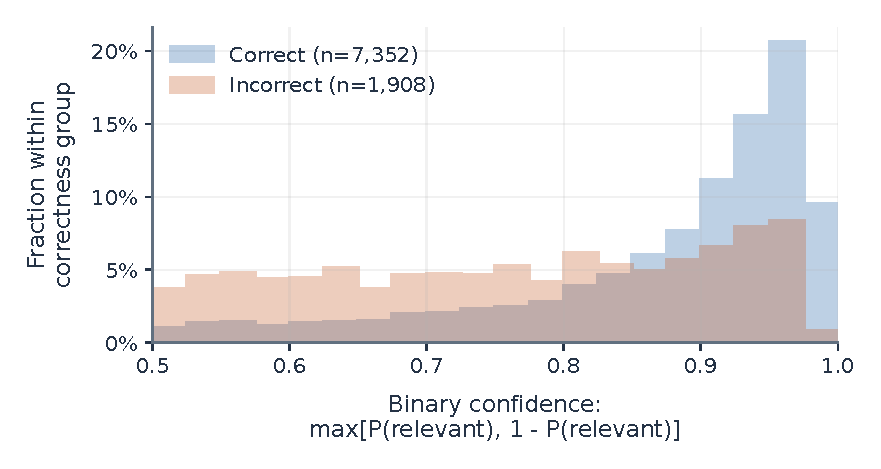
\includegraphics[width=.78\textwidth]{confidence_distribution.pdf}
\caption{Confidence distributions normalized separately within correct and incorrect
groups. The overlap shows why confidence alone cannot perfectly identify errors.
Of the 1,908 errors, 453 have confidence at least 0.90.}
\end{figure}

\begin{figure}[H]\centering
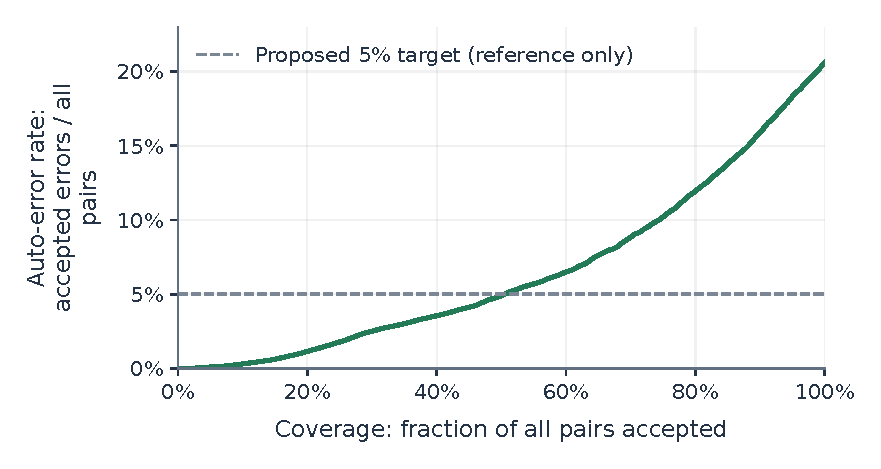
\includegraphics[width=.64\textwidth]{auto_error_coverage.pdf}
\caption{Accepted errors divided by all 9,260 pairs. Unlike selective risk, this
quantity falls mechanically when fewer pairs are accepted. The 5\% line is a
reference target, not a calibrated guarantee.}
\end{figure}

\begin{figure}[H]\centering
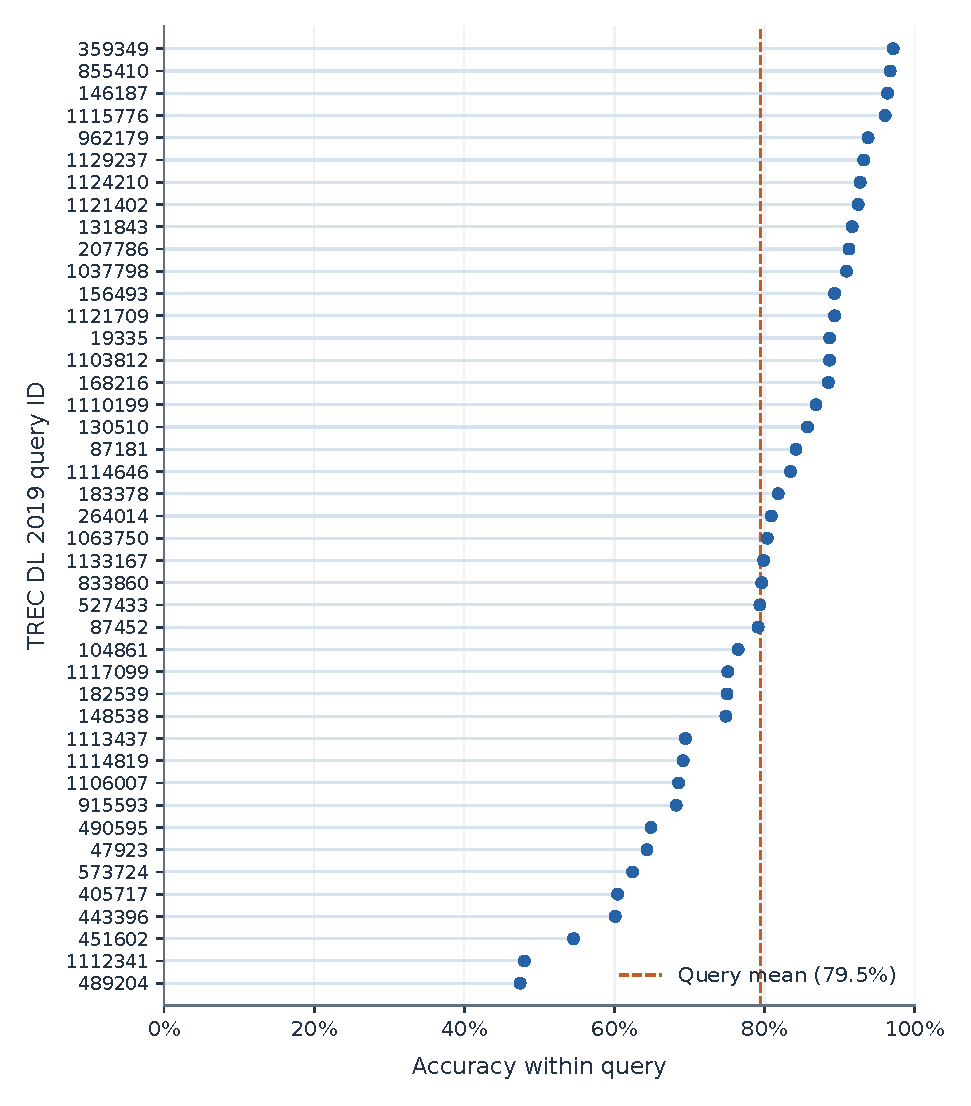
\includegraphics[width=.80\textwidth]{query_accuracy.pdf}
\caption{Accuracy for every query, ordered by observed accuracy. The dashed line
is the equal-query mean (\PilotQueryAccuracy\%). Queries have different judged-pool
sizes and label prevalences; these points are descriptive and have no per-query
confidence intervals.}
\end{figure}
\end{document}
